\chapter{Beyond adversarial loss function}

The Fin-GAN paper \cite{forgan:fin_gan} identifies specific triggers and solutions for these performance issues caused by mode collapse in the ForGAN model. The key findings include:
\begin{itemize}
    \item Weight Initialisation: Using He initialisation led to mode collapse in 67\% of simulations for ForGAN; however, switching to Xavier initialisation significantly alleviated the problem.
    \item Loss Function Regularization: Including standard supervised terms like Mean Squared Error (MSE) or Sharpe Ratio (SR) with high coefficients can actually induce mode collapse by encouraging the model to only output values close to the target.
    \item The paper suggests that adding a Profit and Loss (PnL) term to the generator's loss function acts as an effective regularizer. This term shifts the generated distributions and prevents the model from collapsing into single-point estimates, ensuring a more robust probabilistic forecast.
\end{itemize}

Also in \cite{srforgan:srforgan}, the authors propose replacing the adversarial loss with a strictly proper scoring rule, specifically the Energy Score, which is designed to directly optimize the generator for accurate probabilistic forecasting.
This approach addresses the fundamental issues of mode collapse and training instability by providing a theoretically sound objective that encourages the generator to produce well-calibrated distributions rather than just realistic samples.\\

In particular, the paper proposes replacing the adversarial objective with a scoring rule, which is a function $S(P^\phi, y)$ 
that takes a forecast distribution $P^\phi$ and a single observed realization $y$ and returns a penalty score where the lower the score, the better the forecast.\\
The key definition is strict propriety. A scoring rule $S$ is strictly proper relative to a class $\mathcal{P}$ if:
$$\mathbb{E}_{y \sim P^*}[S(P^*, y)] < \mathbb{E}_{y \sim P^*}[S(P^\phi, y)] \quad \forall P^\phi \neq P^*$$
So the expected score is uniquely minimized when the forecast distribution equals the true data distribution $P^*$. No other distribution achieves a lower expected score. This is the property that makes a scoring rule the right objective for distribution learning because
it is theoretically guaranteed to converge to the right answer, not just some approximation like the 
GAN objective that minimizes a divergence between distributions which has a similar guarantee in principle, but the GAN only minimizes a variational lower bound of that divergence using a finite-capacity critic, which breaks the guarantee in practice.\\

The paper uses the Energy Score as its primary scoring rule. 
For $\beta \in (0,2)$, with $X, X' \sim P^\phi$ independent draws:
\begin{equation}
    \label{eq:energy_score}
S_E^{(\beta)}(P^\phi, y) = 2 \cdot \mathbb{E}\|X - y\|_2^\beta - \mathbb{E}\|X - X'\|_2^\beta
\end{equation}

This Energy Score is obtained from the general Kernel Score:
\begin{equation*}
    \label{eq:kernel_score} 
    S_k(P^\phi, y) = \mathbb{E}[k(X,X')] - 2\mathbb{E}[k(X,y)]
\end{equation*}

By choosing the negative power kernel $k(x,y) = -\|x - y\|_2^\beta$. 
The Kernel Score is strictly proper whenever $k$ is a positive-definite kernel and $-\|x - y\|_2^\beta$ for $\beta \in (0,2)$ is indeed positive-definite.\\

The Energy Score can be decomposed in two terms:
$$S_E^{(\beta)}(P^\phi, y) = \underbrace{2\mathbb{E}\|X - y\|_2^\beta}_{\text{accuracy term}} - \underbrace{\mathbb{E}\|X - X'\|_2^\beta}_{\text{spread reward}}$$
The accuracy term pulls generated samples toward the truth. The spread reward is subtracted, meaning the optimizer is explicitly penalized for producing a degenerate distribution where $X \approx X'$. 
This is the mechanism that prevents mode collapse: a collapsed distribution has $\|X - X'\| = 0$, contributing nothing to the spread reward, making the total score worse than a properly dispersed distribution. The strictly proper guarantee ensures the only global minimum is at $P^\phi = P^*$.\\

The paper fixes $\beta = 1$ throughout. In 1D, $S_E^{(1)}$ recovers exactly the CRPS (Continuous Ranked Probability Score), which is the standard evaluation metric in probabilistic weather forecasting:
\begin{equation}
    \label{eq:crps}
    \begin{aligned}
        \mathrm{CRPS}(F, y) =& \int_{-\infty}^{\infty} \big(F(x) - \mathbf{1}\{x \ge y\}\big)^2 \, dx\\
        &\text{ or alternatively }\\
      \mathrm{CRPS}(F, y)  =& \mathbb{E}|X - y| - \frac{1}{2}\mathbb{E}|X - X'|
    \end{aligned}
\end{equation}


$S_E$ is defined as an expectation over $P^\phi$, but is not possible to differentiate through a sampling operation.
The reparameterization trick resolves this. Because the generator defines:
$$X = h_\phi(z, \text{condition}), \quad z \sim \mathcal{N}(0, I)$$
the expectation formula can be rewritten as:
$$\mathbb{E}_{X \sim P^\phi}[\|X - y\|] = \mathbb{E}_{z \sim \mathcal{N}}[\|h_\phi(z, c) - y\|]$$
The randomness now lives entirely in $z$, which is fixed before the forward pass. 
The generator $h_\phi$ is deterministic and differentiable with respect to its weights. Automatic differentiation libraries can therefore compute $\nabla_\phi S_E$ exactly.
The unbiased Monte Carlo estimator of the full gradient, as discussed in Appendix C of the paper \cite{srforgan:srforgan} is:
$$\hat{S}_E^{(\beta)}(\{x_j\}_{j=1}^m, y) = \frac{2}{m}\sum_{j=1}^m \|x_j - y\|^\beta - \frac{1}{m(m-1)}\sum_{\substack{j,k=1 \\ k \neq j}}^m \|x_j - x_k\|^\beta$$
where each $x_j = h_\phi(z_j, c)$ with $z_j$ drawn independently. The $\frac{1}{m(m-1)}$ denominator excludes diagonal terms and makes this an unbiased estimator. 
Moreover, the paper proves that exchanging gradient and expectation is valid almost surely under mild conditions on the neural network architecture. This means that minimizing the empirical energy score via SGD gives unbiased gradient estimates of the true objective, so convergence results from standard SGD theory apply.



\begin{figure}[H]
    \centering
    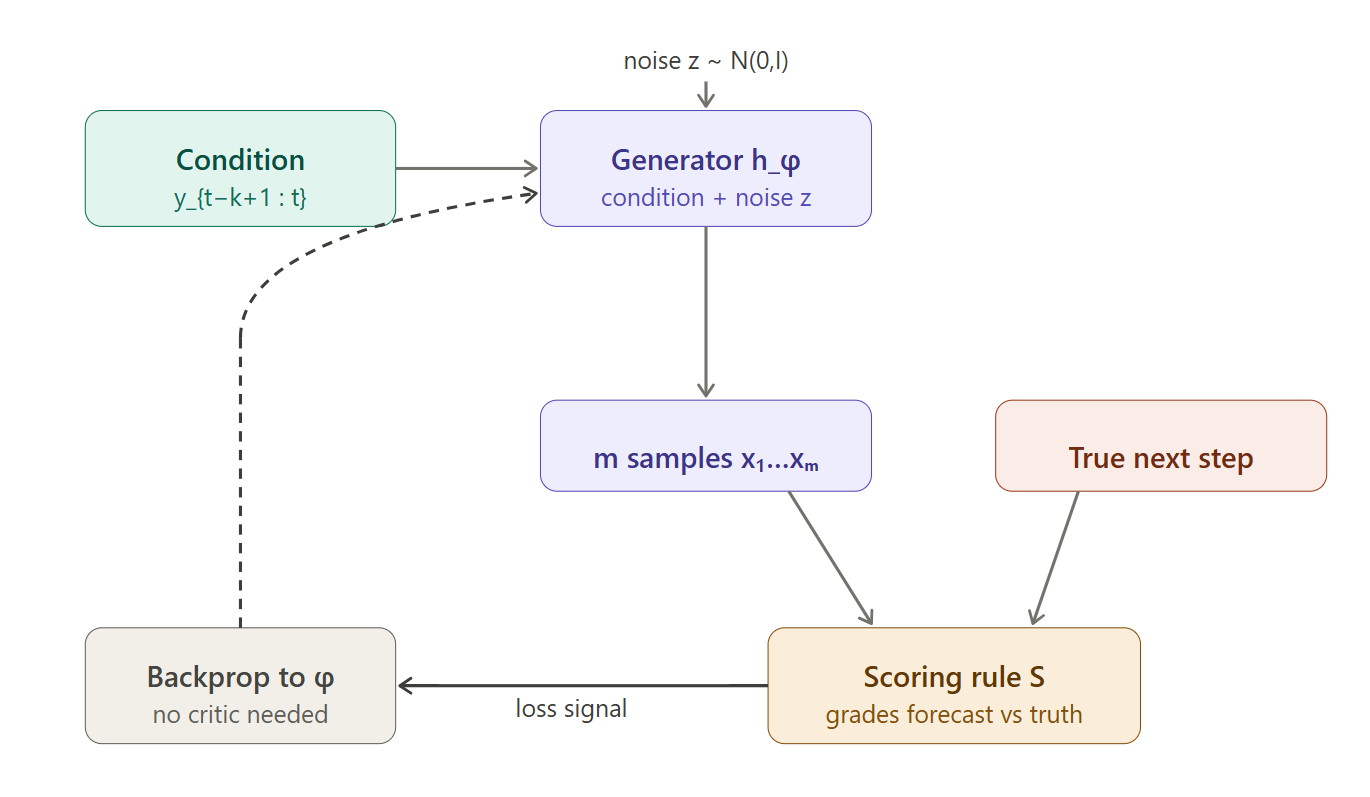
\includegraphics[width=1.0\textwidth]{SRForGAN/images/srforgan_train_schema.png}
    \caption{SRForGAN training schema. The generator takes a noise vector and a conditioning variable to produce a forecast distribution, which is then scored against the true observation using the Energy Score. The critic is not used in this architecture, as the adversarial loss is replaced by the scoring rule objective.}
    \label{img:srforgan_train_schema}
\end{figure}


%
%Layer 5 — The prequential formulation: adapting to time series
%This is the paper's main theoretical contribution. For a temporal sequence $(y_1, \dots, y_T)$, the standard i.i.d. scoring rule objective (Eq. 6 in the paper) is:
%$$\min_\phi \mathbb{E}_{\theta \sim \Pi} \mathbb{E}_{y \sim P^*(\cdot|\theta)} S(P^\phi(\cdot|\theta), y)$$
%This assumes independent context-observation pairs $(\theta_i, y_i)$, which is not true for a time series. The paper replaces this with the prequential (predictive-sequential) score. Given a recorded window of length $T$, forecast each step $l$ ahead conditioned on the previous $k$ observations:
%$$\hat{\phi}_T(y_{1:T}) := \arg\min_\phi \sum_{t=k}^{T-l} S(P^\phi_{t+l}(\cdot|y_{t-k+1:t}),\; y_{t+l})$$
%This is literally how forecasting systems are evaluated in practice: for each time window in your training data, generate a conditional forecast and score it against the realization. The prequential score is then the sum of these one-at-a-time forecasting evaluations across the entire training sequence.
%Why is this still a proper scoring rule despite temporal dependence? The key is Theorem 2 (in the paper): if $S$ is strictly proper, then the prequential score $S_T$ is strictly proper for distributions over $y_{k+l:T}|y_{1:k+l-1}$ that are $k$-Markovian with lag $l$. The proof proceeds by tower property of expectations — propriety at each step propagates to the joint proper scoring of the full sequence. Intuitively, because each term $S(P^\phi_{t+l}(\cdot|y_{t-k+1:t}), y_{t+l})$ depends only on the local window of length $k$, and the generator is the same for all $t$, the sequential evaluation correctly scores the generator's ability to forecast the conditional distribution of the next step.



%Layer 6 — The consistency theorem (Theorem 3)
%This is the rigorous guarantee that makes the method scientifically sound. The empirical minimizer:
%$$\hat{\phi}_T(y_{1:T}) = \arg\min_\phi \frac{1}{T-l-k+1}\sum_{t=k}^{T-l} S(P^\phi(\cdot|y_{t-k+1:t}), y_{t+l})$$
%converges to $\phi^*_T$, the minimizer of the true expected prequential score, as $T \to \infty$, under four assumptions:
%A1 — Compactness: $\Phi$ compact. Standard regularity condition.
%A2 — Uniqueness: The true minimizer is isolated. Lemma 12 shows this is satisfied when $S$ is strictly proper and the model is well-specified (i.e., there exists $\phi^*$ such that $P^{\phi^*} = P^*$).
%A3 — Asymptotic stationarity: The marginal distribution of $(y_{t-k+1:t+l})$ averaged over time converges weakly. This is satisfied for stationary processes like GBM, which has stationary increments.
%A4 — Mixing and moment boundedness: The process is either $\alpha$-mixing or $\phi$-mixing with appropriate decay rates. GBM satisfies $\phi$-mixing since increments are independent. The moment bound for the Energy Score reduces to requiring $\mathbb{E}\|y_{t+l}\|^\beta < \infty$, which holds for log-normal GBM increments.
%The proof combines two classical results: the Uniform Law of Large Numbers for dependent data (Pötscher and Prucha 1989) applied to the sum of scoring rule evaluations, and a generic consistency result (Theorem 5.1, Skouras 1998) which promotes uniform convergence of the objective to convergence of the minimizer. The key insight is that even though consecutive terms in the sum are correlated (since the windows overlap), the mixing condition ensures this dependence decays fast enough that the ULLN still holds. This is fundamentally different from GAN training, which has no analogous consistency result for dependent data.


Additionally, the paper states in the conclusion that the combination of adversarial and SR minimization would be beneficial. So an additional hybrid loss term is added to both the Wasserstein adversarial loss and classical Jensen-Shannon adversarial loss. 
In particular, the generator loss using the hybrid approach is defined as:
\begin{equation}
    \label{eq:hybrid_wasserstein_loss}
    \mathcal{L}_G = \underbrace{-\mathbb{E}[C(G(c,z))]}_{\text{Wasserstein signal}} + \lambda \cdot \underbrace{\hat{S}_E}_{\text{Energy Score}}
\end{equation}







% ── local colour definitions ─────────────────────────────────────────────────
\definecolor{cganblue}{RGB}{30,100,180}
\definecolor{wganred}{RGB}{180,40,40}
\definecolor{commentgray}{RGB}{110,110,110}
 
% ── local math helpers ───────────────────────────────────────────────────────
\newcommand{\Loss}{\mathcal{L}}
\newcommand{\ES}{\hat{S}_{E}}
 
% ── line-comment for the algorithmic package ─────────────────────────────────
% algorithmic has no standalone comment line; emulate it with \STATE
\newcommand{\LINECOMMENT}[1]{%
  \STATE{\color{commentgray}\small$\triangleright$\;\textit{#1}}}
 
% override inline comment style
\renewcommand{\algorithmiccomment}[1]{%
  \hfill{\color{commentgray}\small$\triangleright$\;\textit{#1}}}
 
% ─────────────────────────────────────────────────────────────────────────────
\subsection*{Shared Subroutine — Energy Score Loss}
 
Both models inherit the same \texttt{\_energy\_score\_loss} method.
Given $M$ generator samples $\{\hat{x}_m\}_{m=1}^{M}$ and a batch of
true targets $\mathbf{x} \in \mathbb{R}^{B \times D}$, the unbiased
sample-based Energy Score estimator
(Pacchiardi et al.\ 2024, Appendix C.1.1) is:
 
\begin{equation}
  \ES\!\left(\{\hat{x}_m\}_{m=1}^{M},\,\mathbf{x}\right)
  =
  \underbrace{
    \frac{1}{MB}\sum_{m=1}^{M}\sum_{b=1}^{B}
    \|\hat{x}_m^{(b)} - \mathbf{x}^{(b)}\|_2
  }_{\text{Term 1 --- accuracy}}
  \;-\;
  \underbrace{
    \frac{1}{2\binom{M}{2}B}
    \sum_{\substack{i=1\\j>i}}^{M}
    \sum_{b=1}^{B}
    \|\hat{x}_i^{(b)} - \hat{x}_j^{(b)}\|_2
  }_{\text{Term 2 --- spread reward}}
  \label{eq:es}
\end{equation}
 
The upper-triangle restriction ($j > i$) excludes diagonal
self-differences and yields an \emph{unbiased} estimator with
$\binom{M}{2} = M(M-1)/2$ unique pairs.
 
\begin{algorithm}[H]
\caption{\textsc{EnergyScoreLoss}$\!\left(
  \{\hat{x}_m\}_{m=1}^{M},\;\mathbf{x}\right)$
  --- shared by \texttt{MyCGAN} and \texttt{MyCWGAN}}
\begin{algorithmic}[1]
\REQUIRE $\{\hat{x}_m\}_{m=1}^{M}$: list of $M$ generator outputs,
         each of shape $[B \times D]$
\REQUIRE $\mathbf{x}$: batch of true targets, shape $[B \times D]$
\ENSURE  Scalar Energy Score $\in [0,+\infty)$;
         equals $0$ iff $P^{\phi} = P^{*}$
 
\LINECOMMENT{Stack all M samples into one tensor}
\STATE $\mathbf{S} \leftarrow
  \mathrm{Stack}(\hat{x}_1,\ldots,\hat{x}_M)$
  \COMMENT{shape $[M \times B \times D]$}
 
\LINECOMMENT{Term 1: mean L2 distance from each sample to the truth}
\STATE $T_1 \leftarrow
  \dfrac{1}{M \cdot B}
  \displaystyle\sum_{m=1}^{M}\sum_{b=1}^{B}
  \bigl\|\mathbf{S}[m,b,:] - \mathbf{x}[b,:]\bigr\|_2$
 
\LINECOMMENT{Term 2: mean pairwise L2 distance, upper triangle only}
\STATE $\mathcal{P} \leftarrow [\;]$
\FOR{$i = 1$ \textbf{to} $M$}
  \FOR{$j = i+1$ \textbf{to} $M$}
    \STATE $d_{ij} \leftarrow
      \dfrac{1}{B}\displaystyle\sum_{b=1}^{B}
      \bigl\|\mathbf{S}[i,b,:] - \mathbf{S}[j,b,:]\bigr\|_2$
    \STATE $\mathcal{P}.\mathrm{append}(d_{ij})$
  \ENDFOR
\ENDFOR
\STATE $T_2 \leftarrow
  \dfrac{0.5}{\binom{M}{2}}
  \displaystyle\sum_{d\,\in\,\mathcal{P}} d$
  \COMMENT{$\binom{M}{2}$ unique pairs, diagonal excluded}
 
\RETURN $T_1 - T_2$
  \COMMENT{subtract spread reward to penalise collapse}
\end{algorithmic}
\end{algorithm}
 
\newpage
 
% ─────────────────────────────────────────────────────────────────────────────
\subsection*{{\color{cganblue}Algorithm 1 ---
  \texttt{MyCGAN} Hybrid Generator Update}}
 
The adversarial term uses Binary Cross-Entropy (BCE).
The full hybrid generator loss for one mini-batch is:
 
\begin{equation}
  \Loss_{G}^{\mathrm{CGAN}}
  =
  \underbrace{
    -\frac{1}{B}\sum_{b=1}^{B}
    \log D\!\left(\hat{x}_1^{(b)},\,c^{(b)}\right)
  }_{\text{BCE adversarial loss}}
  \;+\;
  \lambda\;
  \underbrace{
    \ES\!\left(\{\hat{x}_m\}_{m=1}^{M},\,\mathbf{x}\right)
  }_{\text{Energy Score (Eq.\,\ref{eq:es})}}
  \label{eq:cgan_hybrid}
\end{equation}
 
\begin{algorithm}[H]
\caption{{\color{cganblue}\texttt{MyCGAN}} --- hybrid generator update
  (called when $\mathrm{step} \bmod n_{\mathrm{critic}} = 0$)}
\begin{algorithmic}[1]
\REQUIRE Generator $G_{\phi}$, Discriminator $D_{\psi}$
\REQUIRE Condition batch $\mathbf{c}$, true targets $\mathbf{x}$,
         real labels $\mathbf{1}$, samples $M$,
         ES weight $\lambda$, noise dim $N_z$
\ENSURE  Updated generator parameters $\phi$
 
\STATE $\mathrm{ZeroGrad}(\phi)$
 
\LINECOMMENT{Draw M independent noise vectors; generate M samples}
\STATE $\mathrm{samples} \leftarrow [\;]$
\FOR{$m = 1$ \textbf{to} $M$}
  \STATE $\mathbf{z}_m \sim \mathcal{N}(\mathbf{0},\,\mathbf{I}_{N_z})$
  \COMMENT{fresh draw each iteration}
  \STATE $\hat{x}_m \leftarrow G_{\phi}(\mathbf{c},\,\mathbf{z}_m)$
  \COMMENT{shape $[B \times D]$}
  \STATE $\mathrm{samples}.\mathrm{append}(\hat{x}_m)$
\ENDFOR
 
\LINECOMMENT{Adversarial term: pass only the first sample through D}
\STATE $\mathrm{logits}
  \leftarrow D_{\psi}\!\left(\mathrm{samples}[1],\,\mathbf{c}\right)$
\STATE $\Loss_{\mathrm{adv}}
  \leftarrow \mathrm{BCE}(\mathrm{logits},\;\mathbf{1})$
  \COMMENT{generator wants $D$ to output 1 on fakes}
 
\LINECOMMENT{Energy Score term: all M samples contribute}
\STATE $\Loss_{\mathrm{ES}}
  \leftarrow
  \textsc{EnergyScoreLoss}(\mathrm{samples},\;\mathbf{x})$
 
\LINECOMMENT{Combine, backpropagate once, update}
\STATE $\Loss_{G}
  \leftarrow \Loss_{\mathrm{adv}} + \lambda \cdot \Loss_{\mathrm{ES}}$
\STATE $\mathrm{Backward}(\Loss_{G})$
  \COMMENT{gradients from both terms accumulate in one pass}
\STATE $\mathrm{Step}(\phi)$
\RETURN $\Loss_{G}$
\end{algorithmic}
\end{algorithm}
 
\textbf{Note.}\;
$\hat{x}_1 = \mathrm{samples}[1]$ contributes to \emph{both}
$\Loss_{\mathrm{adv}}$ (through $D_\psi$) and
$\Loss_{\mathrm{ES}}$ (as element $m=1$ inside
\textsc{EnergyScoreLoss}).
PyTorch accumulates both gradient contributions correctly in a single
\texttt{backward()} call.
 
\newpage
 
% ─────────────────────────────────────────────────────────────────────────────
\subsection*{{\color{wganred}Algorithm 2 ---
  \texttt{MyCWGAN} Hybrid Generator Update}}
 
The adversarial term is the Wasserstein generator loss
$-\mathbb{E}[C(\hat{x})]$; no labels are needed since the critic
output is an unbounded real score.
 
\begin{equation}
  \Loss_{G}^{\mathrm{CWGAN}}
  =
  \underbrace{
    -\frac{1}{B}\sum_{b=1}^{B}
    C\!\left(\hat{x}_1^{(b)},\,c^{(b)}\right)
  }_{\text{Wasserstein generator loss}}
  \;+\;
  \lambda\;
  \underbrace{
    \ES\!\left(\{\hat{x}_m\}_{m=1}^{M},\,\mathbf{x}\right)
  }_{\text{Energy Score (Eq.\,\ref{eq:es})}}
  \label{eq:cwgan_hybrid}
\end{equation}
 
\begin{algorithm}[H]
\caption{{\color{wganred}\texttt{MyCWGAN}} --- hybrid generator update
  (called when $\mathrm{step} \bmod n_{\mathrm{critic}} = 0$)}
\begin{algorithmic}[1]
\REQUIRE Generator $G_{\phi}$, Critic $C_{\psi}$
\REQUIRE Condition batch $\mathbf{c}$, true targets $\mathbf{x}$,
         samples $M$, ES weight $\lambda$, noise dim $N_z$
\ENSURE  Updated generator parameters $\phi$
 
\STATE $\mathrm{ZeroGrad}(\phi)$
 
\LINECOMMENT{Draw M independent noise vectors; generate M samples}
\STATE $\mathrm{samples} \leftarrow [\;]$
\FOR{$m = 1$ \textbf{to} $M$}
  \STATE $\mathbf{z}_m \sim \mathcal{N}(\mathbf{0},\,\mathbf{I}_{N_z})$
  \STATE $\hat{x}_m \leftarrow G_{\phi}(\mathbf{c},\,\mathbf{z}_m)$
  \COMMENT{shape $[B \times D]$}
  \STATE $\mathrm{samples}.\mathrm{append}(\hat{x}_m)$
\ENDFOR
 
\LINECOMMENT{Wasserstein term: no labels; maximise critic score on fakes}
\STATE $\Loss_{\mathrm{W}}
  \leftarrow
  -C_{\psi}\!\left(\mathrm{samples}[1],\,\mathbf{c}\right).\mathrm{mean}()$
  \COMMENT{no target labels required}
 
\LINECOMMENT{Energy Score term: all M samples contribute}
\STATE $\Loss_{\mathrm{ES}}
  \leftarrow
  \textsc{EnergyScoreLoss}(\mathrm{samples},\;\mathbf{x})$
 
\LINECOMMENT{Combine, backpropagate once, update}
\STATE $\Loss_{G}
  \leftarrow \Loss_{\mathrm{W}} + \lambda \cdot \Loss_{\mathrm{ES}}$
\STATE $\mathrm{Backward}(\Loss_{G})$
\STATE $\mathrm{Step}(\phi)$
\RETURN $\Loss_{G}$
\end{algorithmic}
\end{algorithm}
 
% ─────────────────────────────────────────────────────────────────────────────
\subsection*{Critic / Discriminator Update (unchanged in both models)}
 
The critic is trained on \texttt{detach()}ed fake samples and does
not interact with the Energy Score in any way.
 
\begin{equation}
  \Loss_{D}^{\mathrm{CGAN}}
  = -\mathbb{E}[\log D(\mathbf{x},\mathbf{c})]
    -\mathbb{E}[\log(1 - D(\hat{x},\mathbf{c}))]
\end{equation}
\begin{equation}
  \Loss_{C}^{\mathrm{CWGAN}}
  = -\mathbb{E}[C(\mathbf{x},\mathbf{c})]
    +\mathbb{E}[C(\hat{x},\mathbf{c})]
    +\lambda_{\mathrm{GP}}\cdot
    \mathrm{GP}(\mathbf{x},\hat{x},\mathbf{c})
\end{equation}
 
% ─────────────────────────────────────────────────────────────────────────────
\subsection*{Structural Comparison}
 
\begin{center}
\renewcommand{\arraystretch}{1.45}
\begin{tabular}{lcc}
\toprule
Property
  & {\color{cganblue}\textbf{MyCGAN}}
  & {\color{wganred}\textbf{MyCWGAN}} \\
\midrule
Adversarial term
  & $-\mathbb{E}[\log D(\hat{x},c)]$
  & $-\mathbb{E}[C(\hat{x},c)]$ \\
Discriminator output
  & sigmoid $\in(0,1)$
  & unbounded $\in(-\infty,+\infty)$ \\
Labels needed
  & yes ($\mathbf{1}$ for fakes)
  & no \\
Critic regularisation
  & none
  & gradient penalty (GP) \\
Energy Score term
  & $\ES(\{\hat{x}_m\},\mathbf{x})$
  & $\ES(\{\hat{x}_m\},\mathbf{x})$ \\
ES implementation
  & \multicolumn{2}{c}{%
      identical --- shared \texttt{\_energy\_score\_loss}} \\
Early stopping metric
  & not implemented
  & $\Loss_{\mathrm{W}} + \lambda\Loss_{\mathrm{ES}}$ \\
Better metric direction
  & \multicolumn{2}{c}{lower is better
    ($\Loss_{\mathrm{ES}}\geq 0$;
     $\Loss_{\mathrm{W}}\leq 0$ when generator is strong)} \\
\bottomrule
\end{tabular}
\end{center}